\documentclass[twocolumn,9pt]{jsproceedings}
\RequirePackage[l2tabu,orthodox]{nag}  % 古いコマンドやパッケージを使用した場合に警告する
%\usepackage{subcaption}
\usepackage[all,warning]{onlyamsmath}  % amsmath が提供しない数式環境を使用した場合に警告する
% \usepackage{flushend}  % 最終ページの2カラムの左右の高さを揃える
\usepackage{here} %図の場所の指定で[h](ここに貼る)を指定するためのパッケージ
\usepackage[dvipdfmx]{graphicx} %dvipdfmxはjpgやpngの張り込みのために使用
%\usepackage{graphicx}

% タイトル
\title{小型自律移動ロボットを用いた\\つくばチャレンジ2023での取り組み}

\author{○池邉 龍宏\authorrefmark{2}、内田 璃空\authorrefmark{2}、畑中 優一郎\authorrefmark{2}、吉越 誠\authorrefmark{1}、臼井 温希\authorrefmark{1}、庄司 史門\authorrefmark{1}、
\\青木 優羽\authorrefmark{1}、藤崎 賢蔵\authorrefmark{1}、川原 脩慈\authorrefmark{1}、三浦 璃音\authorrefmark{1}、永木 悠暉\authorrefmark{1}、茂 郁良\authorrefmark{1}、
\\佐々木 新平\authorrefmark{1}、林原 靖男\authorrefmark{1}、上田 隆一\authorrefmark{1}}

%\etitle{Participation report in the Tsukuba Challenge 2023\\using a small mobile robot}
\etitle{Development for Tsukuba Challenge 2023\\with small mobile robots}

\eauthor{○Tatsuhiro IKEBE\eauthorrefmark{2}、Riku UCHIDA\eauthorrefmark{2}、Yuichiro HATANAKA\eauthorrefmark{2}、Makoto YOSHIGOE\eauthorrefmark{1}、\\Atsuki USUI\eauthorrefmark{1}、Shimon SHOJI\eauthorrefmark{1}、
Yuwa AOKI\eauthorrefmark{1}、Kenzo FUJISAKI\eauthorrefmark{1}、Yuzi KAWAHARA\eauthorrefmark{1}、\\Rion MIURA\eauthorrefmark{1}、Yuki NAGAKI\eauthorrefmark{1}、Ikuo SHIGE\eauthorrefmark{1}、Shinpei SASAKI\eauthorrefmark{1}、\\Yasuo HAYASHIBARA\eauthorrefmark{1}、Ryuichi UEDA\eauthorrefmark{1}}

\affiliation{千葉工業大学 未来ロボティクス学科 ツナチーム/たまチーム/むぎまるチーム}

\begin{document}
\maketitle

\authorreftext{1}{千葉工業大学先進工学部未来ロボティクス学科}
\authorreftext{2}{千葉工業大学院先進工学研究科未来ロボティクス専攻}
\eauthorreftext{1}{Department of Advanced Robotics、Faculty of Advanced Engineering、Chiba Institute of Technology}
\eauthorreftext{2}{Department of Advanced Robotics、Graduate School of Advanced Engineering、Chiba Institute of Technology}

% 本文
\section{緒言}

千葉工業大学未来ロボティクス学科上田研究室では、
「屋外で小型移動ロボットが安全に自律移動するためのシステムの構築」を目的として、
2021年からつくばチャレンジに参加してきた。
つくばチャレンジ2023には、
チームからは「ツナチーム」、「たまチーム」、「むぎまるチーム」
という名義で計3チームがエントリーした。
%小型な移動ロボットをあえて使用する動機は、
%他のチームでは見つけることのできない、小型移動ロボットならではの
%問題を発見、解決するためである。




各チームの具体的な目標は、
\begin{itemize}
  \item ツナチーム:ROS 2実装での自作ナビゲーションスタックを小型ロボットで実用
  \item たまチーム:本研究室の自己位置推定パッケージであるemcl2\cite{emcl2}をROS 2に移行したemcl2\_ros2\cite{emcl2_ros2}と、Nav2を組み合わせて小型ロボットで実用
  \item むぎまるチーム:安価・小型な3次元LiDARを用いた自律移動システムを小型ロボットで実用
\end{itemize}
であった。


本稿では、各チームで立てた目標に対する取り組みと結果について説明する。
本稿の構成は次の通りである。
2章ではロボットのソフトウェア、ハードウェア構成について説明し、
3章では本走行の結果と見つかった課題を示す。
4章では結言を述べる。

\section{各チームのロボットの構成}

各チームのロボットの外観を図\ref{fig:robot}に示す。
いずれも、アールティ社製の既製品である
Raspberry Pi Cat\cite{RTshop}がベースになっている。
もともとのRaspberry Pi Catには全面の保護カバーが
ないが、いずれのチームも、図のように3Dプリンターで
カバーを作成し、取り付けて参加した。
また、レギュレーションの関係で、
アルミフレームで台車の持ち手のような構造物を組み、
その上に非常停止ボタンを取り付けてある。



計算機については、ノートPCを各ロボットに搭載して使用した。
昨年は、1チームが計算機としてRaspberry Pi 4 Model Bのみを
使用して自律走行を実現した\cite{池邉2022}。
しかし本年度については、
Raspberry Pi上でROS 2を実行するための
技術的な課題が解決しておらず、
ノートPCを使用することとなった。
この場合、Raspberry Pi Catには、
ノートPCと制御用のRaspberry Piの2台の計算機が搭載されることとなる。
センサ構成としては、各チームの機体に外界センサとして
2次元LiDAR、3次元LiDAR、内界センサとしてIMUを搭載した。

% \begin{figure}[H]
%   \begin{minipage}[b]{0.48\columnwidth}
%     \centering
%     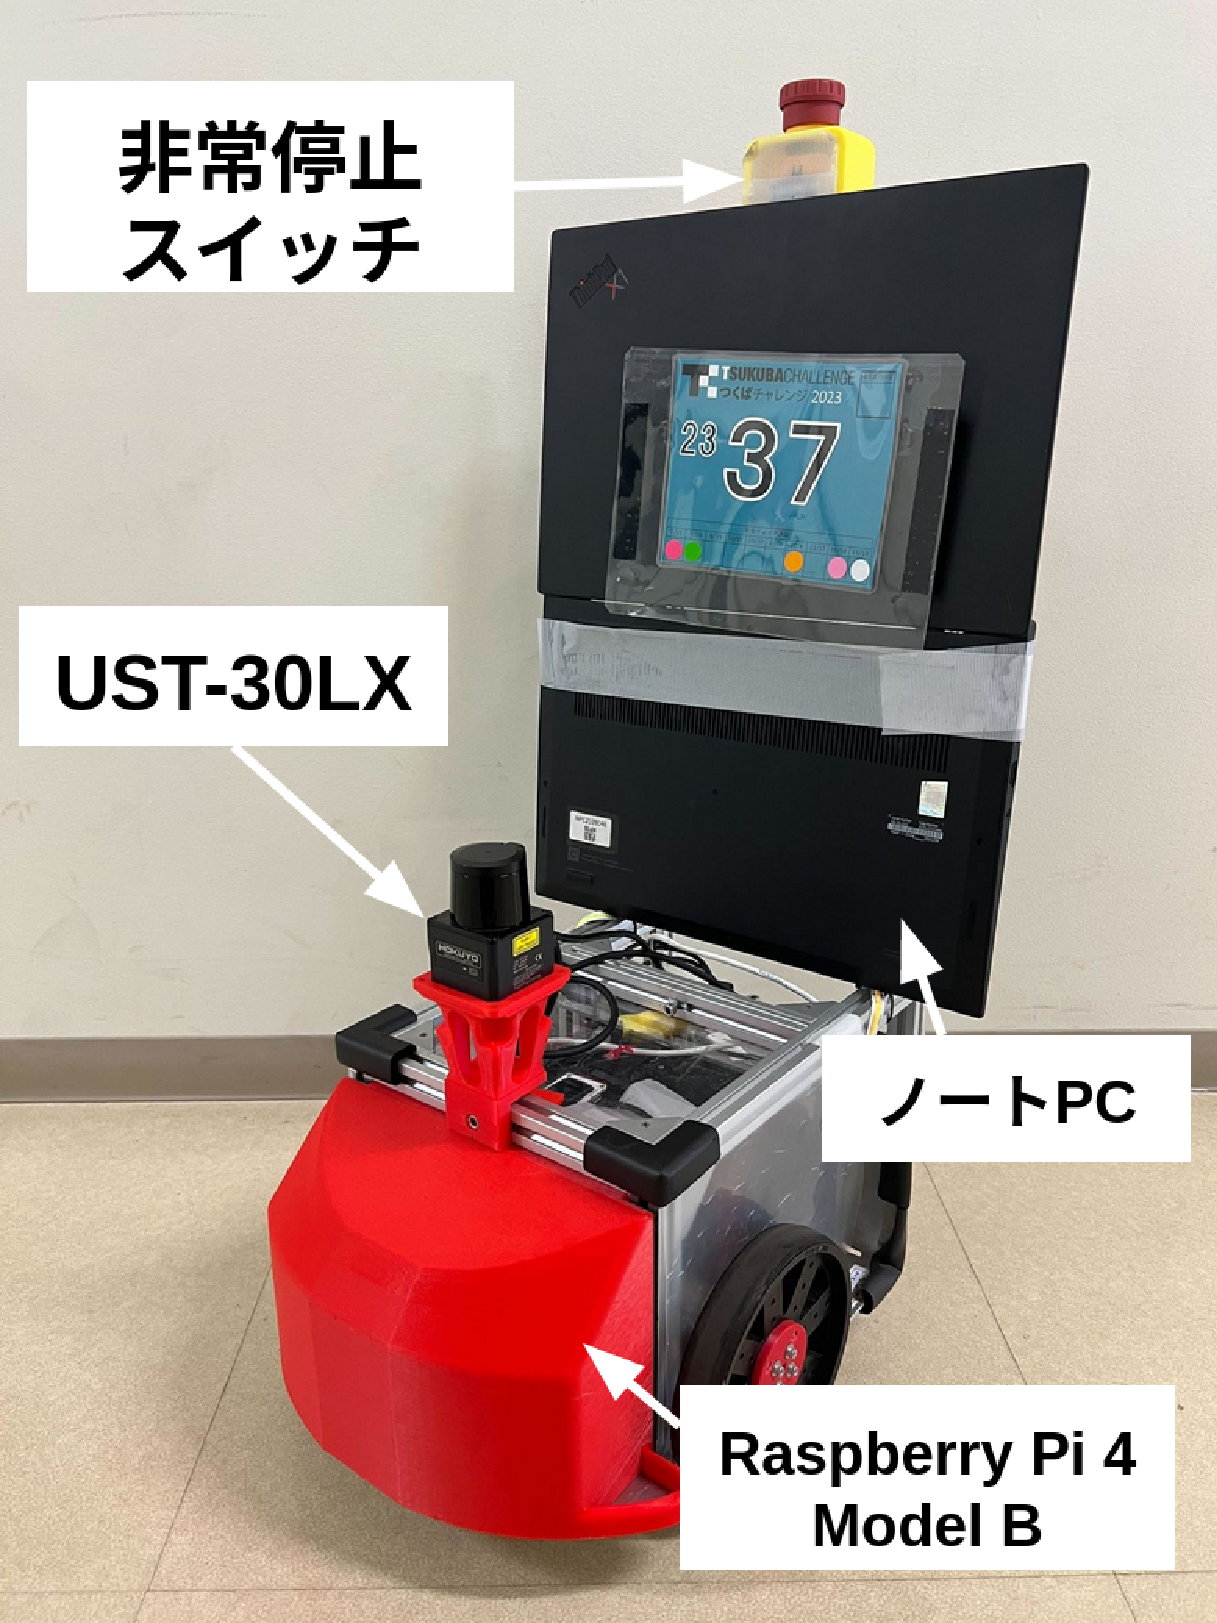
\includegraphics[width=1.0\linewidth]{figs/tuna_robot.pdf}
%     \caption{ツナチームの機体}
%     \label{tuna}
%   \end{minipage}
%   \hspace{0.04\columnwidth} % ここで隙間作成
%   \begin{minipage}[b]{0.48\columnwidth}
%     \centering
%     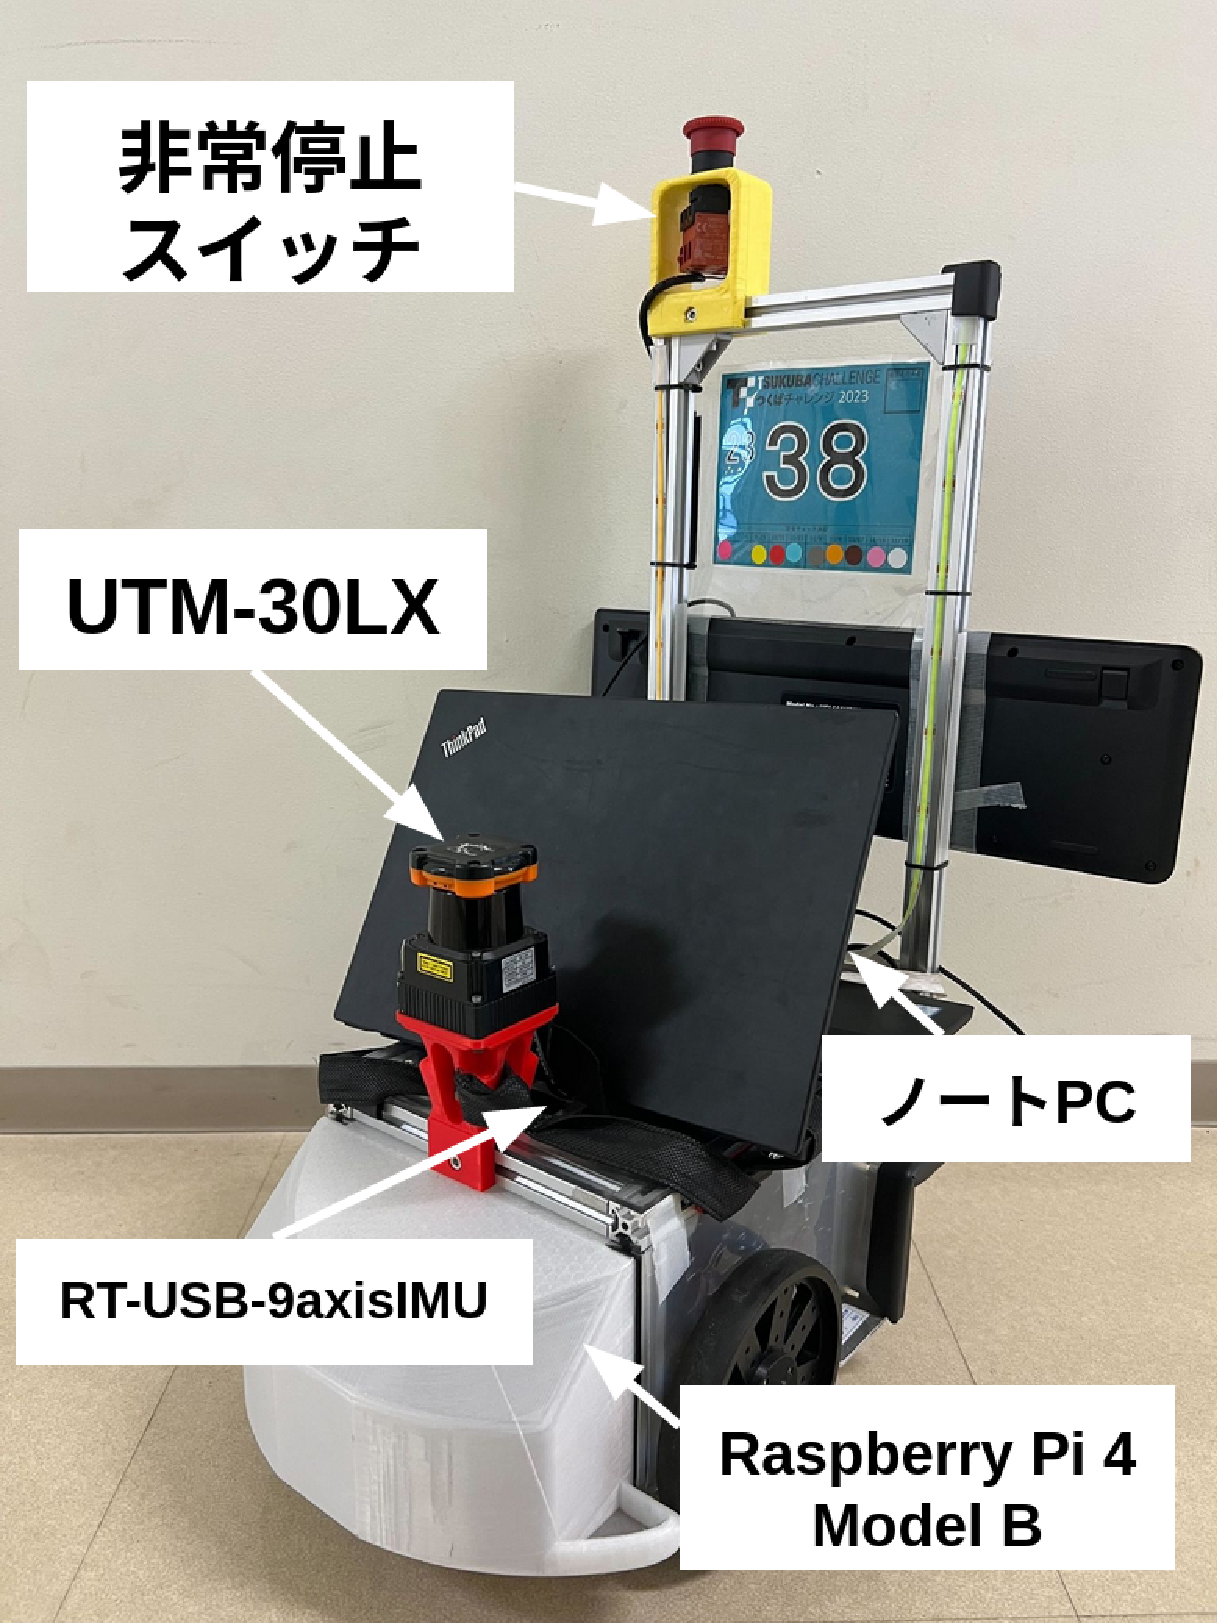
\includegraphics[width=1.0\linewidth]{figs/tama_robot.pdf}
%     \caption{たまチームの機体}
%     \label{tama}
%   \end{minipage}\\
%   \begin{minipage}[b]{0.48\columnwidth}
%     \centering
%     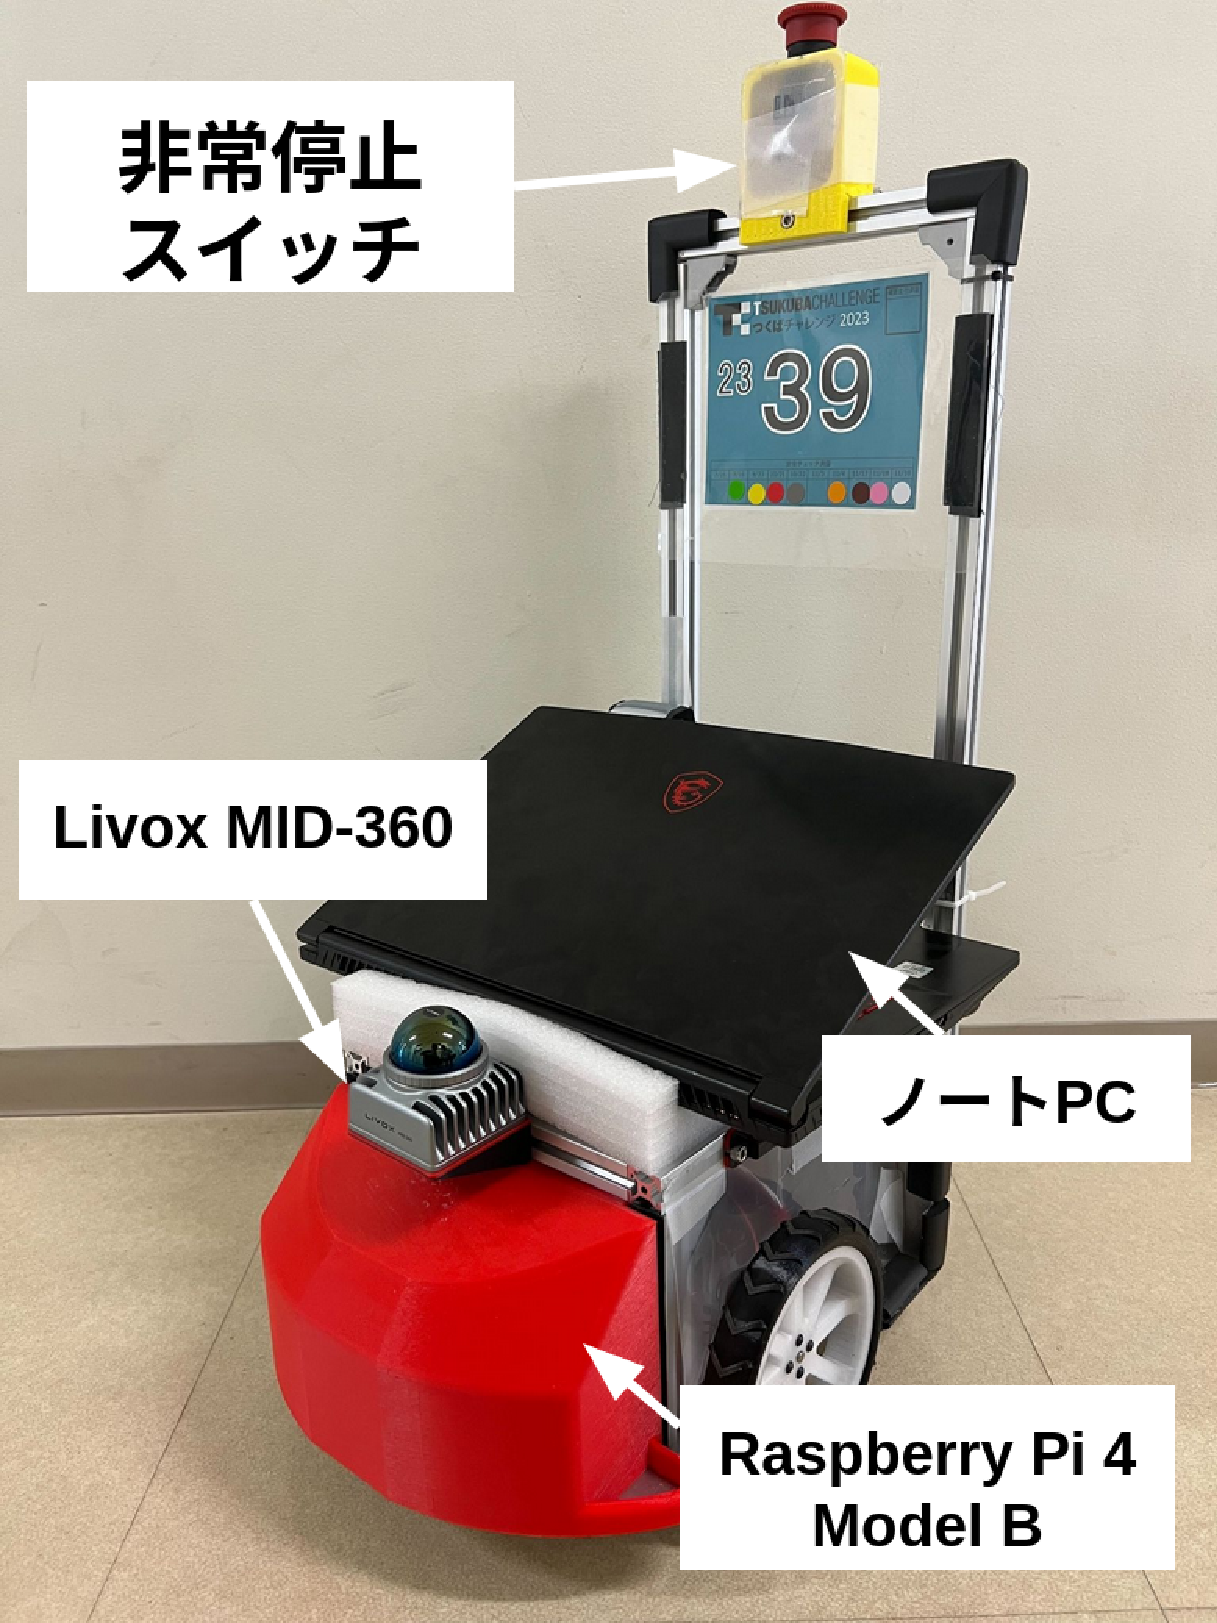
\includegraphics[width=1.0\linewidth]{figs/mugimaru_robot.pdf}
%     \caption{むぎまるチームの機体}
%     \label{mugi}
%   \end{minipage}
% \end{figure}

\begin{figure}[h]
  \begin{center}
    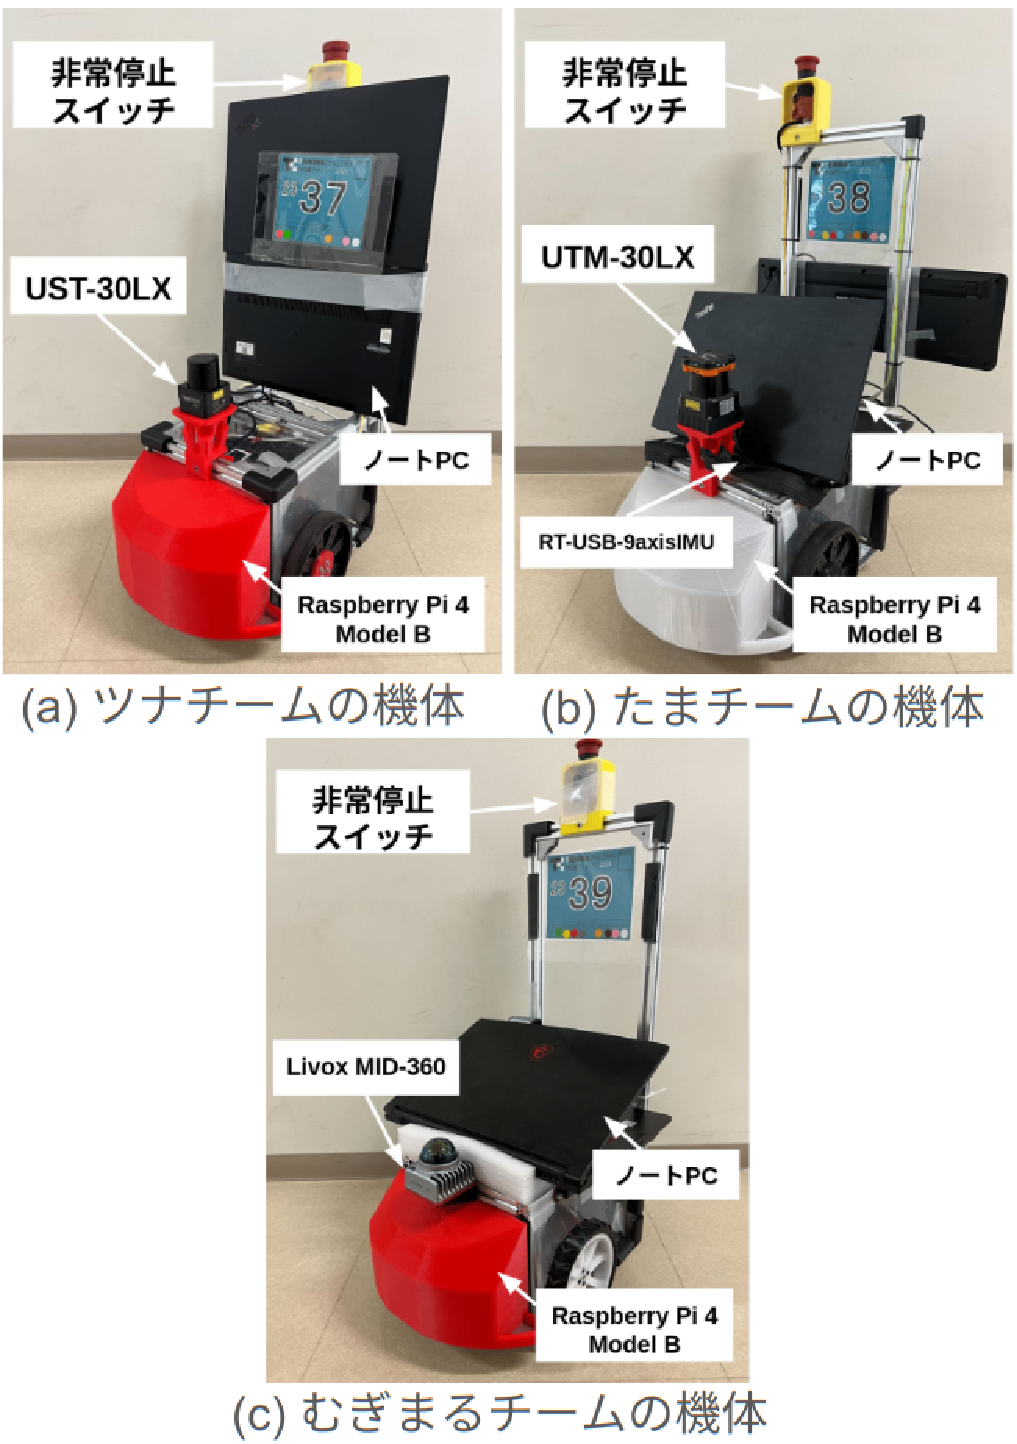
\includegraphics[width=1.0\linewidth]{figs/robot.pdf}
    \caption{各チームの機体}
    \label{fig:robot}
  \end{center}
\end{figure}

ソフトウェアについては、
本年度は、3チーム全てがROS 2\cite{ROS 2}をベースに構築した。
昨年度まではROS\cite{ROS}を使用していたが、
ROSの最終リリースであるROS Noetic Ninjemysが2025年5月に
サポート終了を迎えることを受けてのことである。

他、各チームの特徴について、
次節以降で説明する。


\subsection{ツナチーム}


\subsubsection{概要}
ツナチームは、ROS 2をベースに自作ナビゲーションスタックを自作し、
%図\ref{fig:robot}の小型移動ロボット上で動作させ、
自律走行させた。
%をさせることを目的とした。
作成した自作ナビゲーションスタックは、
GitHub上のリポジトリuhobeike/ike\_nav\cite{ike_nav}
に公開している。
また、リポジトリの内容については
%「自作ナビゲーションスタックでつくばチャレンジ2023に挑戦してみた話」
\cite{ike_nav_detail}にまとめた。
%↑いちおう教育的観点で言うと、「記事内に金出した研究室とかその他関係者に謝辞入れやがれ自分のことしか書いてなくてよくないよこれ。」
%(言うの恥ずかしいので言わせないでほしい・・・)

このパッケージは、「Nav2のような複雑な
システムではなく、シンプルで修正しやすいパッケージを作成したい」
という動機で作成した。
ソフトウェアを再利用して巨人の肩に乗ることは重要であるが、
ブラックボックスのない
ソフトウェアパッケージを開発する方針も考えられたため、
開発に踏み切った。

%例えば、つくばチャレンジ中に何か解決したい問題が発生し、
%ソフトウェア上で解決したいとなった場合に、
%パラメータやコードに対して手を入れやすいメリットがあると考えている。

%uhobeike/ike\_navの作成に関する詳細については、

%↓いらない
%\subsubsection{使用したハードウェア}
%ツナチームでは、図\ref{fig:robot}の機体を自律走行させた。
%機体には、2つのコンピュータが搭載されている。
%一つ目は、計算用として、ノートPCを搭載した。
%このノートPC上でike\_navを動作させた。
%二つ目は、機体の制御用として、Raspberry Pi 4B+を搭載した。
%
%観測用のセンサは、2次元LiDARであるUST-30LX\cite{UST-30LX}を搭載した。
%このLiDARの捜査角度は、270[deg]であり、最大検出距離は60[m]である。


\subsubsection{ike\_navのシステム構成}

図\ref{fig:tuna_system}に、ike\_navのシステム構成を示す。
ike\_navは、地図、2次元LiDARからの観測情報(スキャン)、
ロボットのオドメトリを入力して受け入れ、
ある目標地点まで到達するための速度および推定した自己位置を出力する。

\begin{figure}[h]
  \begin{center}
    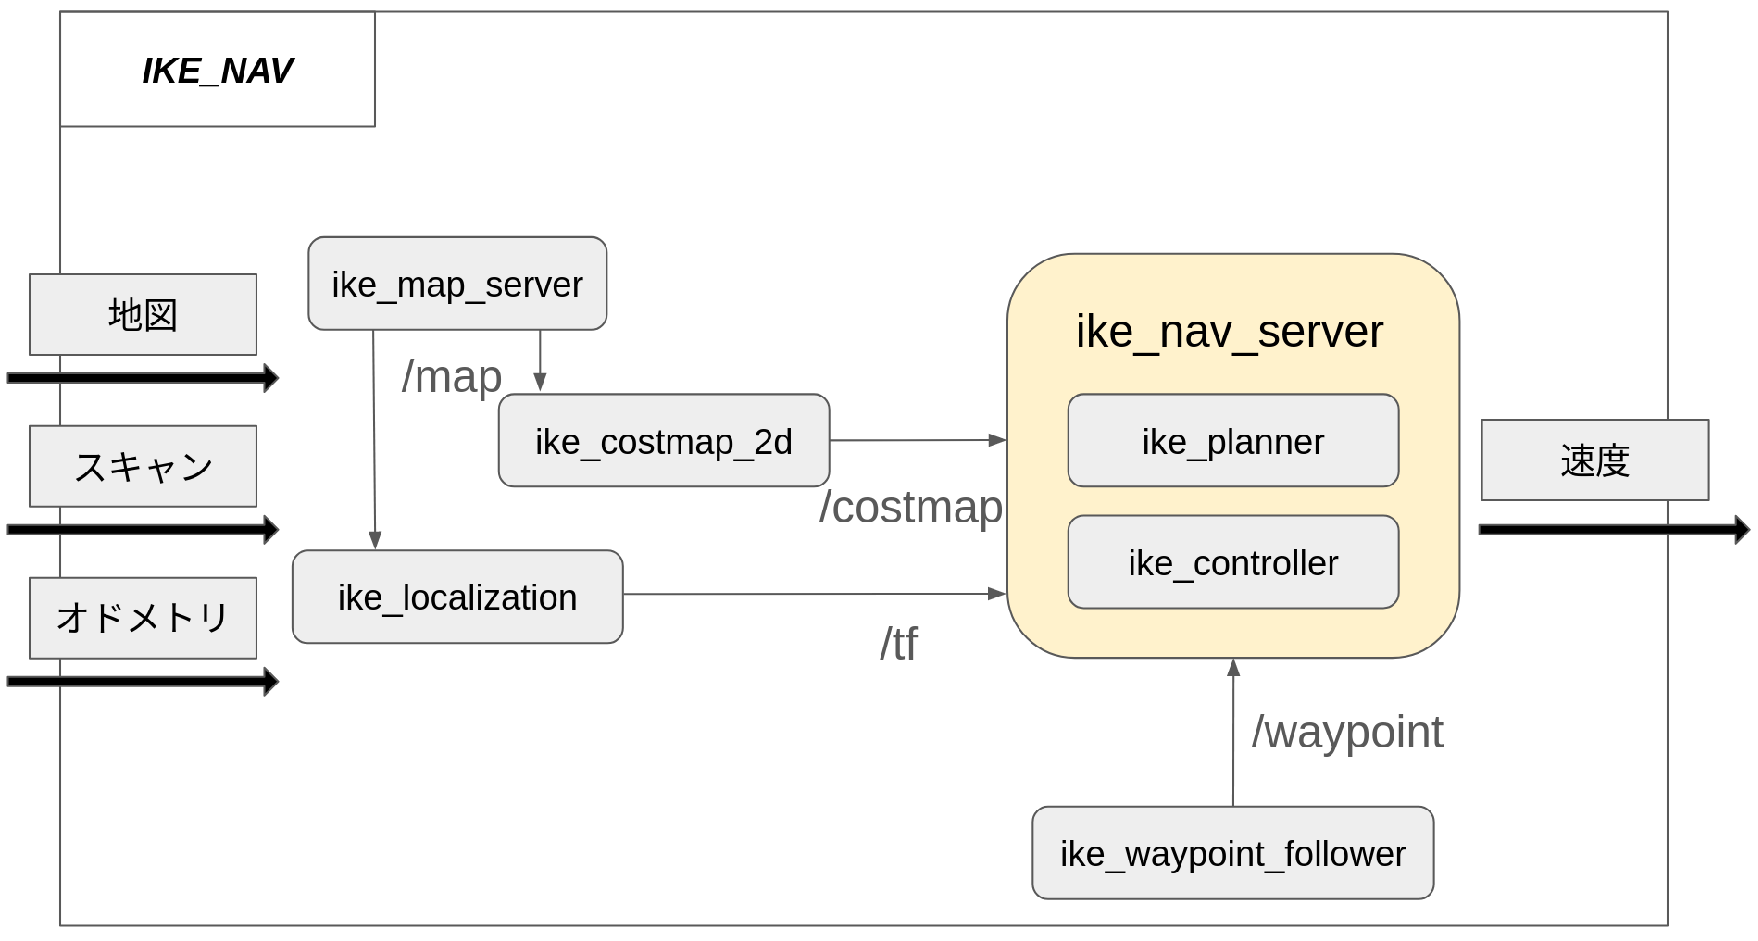
\includegraphics[width=1.0\linewidth]{figs/ike_nav.pdf}
    \caption{ツナチームのシステム構成}
    \label{fig:tuna_system}
  \end{center}
\end{figure}

ike\_navは、メタパッケージであり、
ロボットの自律走行に必要な技術である、
自己位置推定、経路計画、経路追従などがそれぞれ別々にパッケージ化されている。
ロボットが自律走行をするのに、
強く関わりがあるパッケージを列挙すると以下のとおりである。

\begin{description}
  \item[・ike\_controller(経路追従):]経路、推定位置を入力し、速度を出力
  \item[・ike\_costmap\_2d(コストマップの管理):]地図、観測情報を入力し、コストマップを出力
  \item[・ike\_localization(自己位置推定):]観測情報、地図、ロボットのオドメトリを入力し、自己位置を出力
  \item[・ike\_map\_server(地図の管理):]pgmなどのデータからROS 2の占有格子地図を出力
  \item[・ike\_nav\_server(目標地点までの管理):]目標地点を入力し、到達するまでを管理
  \item[・ike\_planner(経路計画):]コストマップ、推定位置を入力し、経路を出力
  \item[・ike\_waypoint\_follower(複数目標地点の管理):]事前に設定した目標地点を辿るように管理
\end{description}

このうち、主要なパッケージについて詳しく説明する。
まず、ike\_localizationであるが、自己位置推定の手法として、
モンテカルロ自己位置推定法(MCL: Monte Carlo Localization)\cite{fox1999etal}を実装した。
MCLは、比較的実装が容易である上に、
環境における不確実性に強くロバスト性があるため採用をした。
次にike\_planner(経路計画)であるが、経路計画のためにA*\cite{hart1968}を実装した。
A*は、最短経路を導出するアルゴリズムであり、他の最短経路法であるダイクストラ\cite{dijkstra1959}よりも
速く最短経路を導出することができるため採用した。
また実装したA*では、センサから観測した障害物をコストとして、障害物を回避させるような
経路を導出するように実装した。
最後に、ike\_controller(経路追従)であるが、経路追従の手法として、
モデル予測制御(MPC: Model Predictive Control)\cite{alberto2006}を実装した。
MPCは、他の追従手法と比較して、計算コストが高いというデメリットがあるが、
経路に対する追従性が高いというメリットがあるため採用した。


\subsection{たまチーム}\label{sub:localization}
\subsubsection{概要}
たまチームは、ROS 2に移行されたemcl2パッケージemcl2\_ros2を用いて、
屋外でロボットに自律走行させた。
目標に関しては、つくばチャレンジ初参加のチームメンバーであることも考え、
無理に完走を目指さず、交差点手前までのナビゲーションということにした。

\subsubsection{使用したハードウェアとソフトウェア}

たまチームのシステムの構成を図\ref{fig:tama_system_diagram}に示す.
ロボットに搭載された2D LiDARとIMUから、
Raspberry Pi 4B+を介し、センサ情報をノートPCに送信する。
ノートPCでは自己位置推定、経路計画が行われ、
その結果として得られた制御指令がRaspberry Pi 4に返される。
マッピングにはslam\_toolboxを利用し、
経路計画にはNav2を利用した。
また、自己位置推定においては、
昨年度まで利用されていたemcl2パッケージを
ROS 2に移行した、emcl2\_ros2利用している。

\begin{figure}[h]
  \begin{center}
    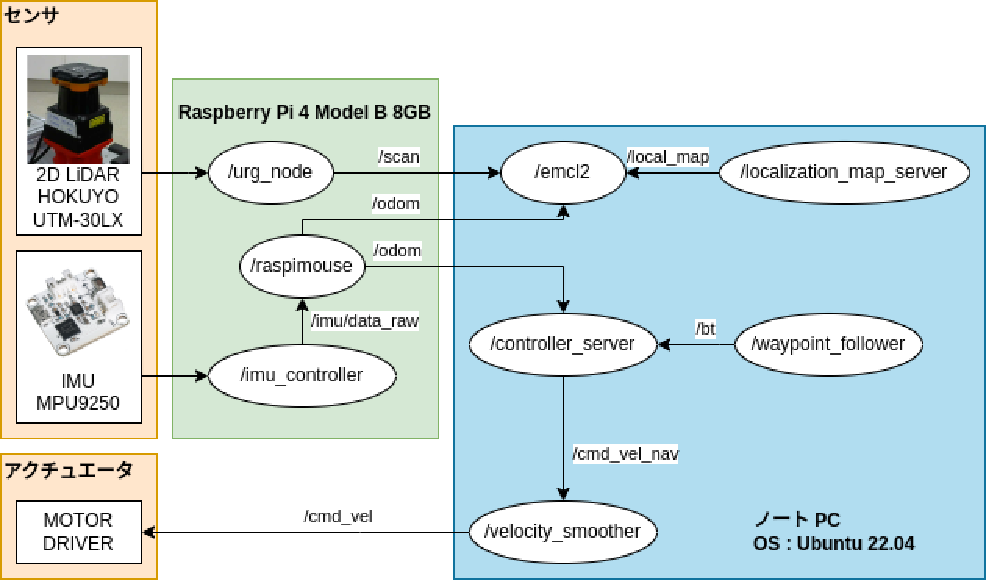
\includegraphics[width=1.0\linewidth]{figs/tama_system_diagram.pdf}
    \caption{たまチームのシステム構成}
    \label{fig:tama_system_diagram}
  \end{center}
\end{figure}

\subsection{むぎまるチーム}

\subsubsection{概要}

むぎまるチームでは,当研究室所属のチームでは始めてとなる,3次元LiDARを用いた
移動ロボットの自律走行に挑戦し,チーム目標には確認走行区間の完走を掲げていた.
%自律走行の方法は,走行区間の環境地図を事前に作成し,3次元LiDARのスキャンデータ
%とのマッチングにより求めた自己位置をもとに自律走行を行うものである.
ソフトウェアはすべて,ROS/ROS 2の上で使用される標準的なパッケージを活用した.
すべて、Ubuntu 22.04上で動作する既存のROS2 Humbleのパッケージであった。

\subsubsection{使用したハードウェアとソフトウェア}

%むぎまるチームが実験走行・本走行で使用したロボットを図xに示す.
%ロボット本体には同所属の他チーム同様,株式会社アールティ様が販売している Raspberry Pi Cat を使用した.
%@@@まず概要を述べてから細かい話をする@@@
むぎまるチームは、
ノートPCとしてMSI製 GF65 Thin 10SERを使用した。
また、制御用Raspberry Piのバージョンは4B+であた。
%Raspberry Piは,速度司令のみをラップトップPCから入力し,
%Raspberry Pi Catを動かすドライバの役割として使用した.
%ノートPCでは自己位置推定,経路生成,経路追従などの主要となる計算を行う役割を担当していた.

センサについては,3D LiDARとしてLivox製のMid-360を使用し,
IMUにはMid-360に内蔵されるICM40609を使用した.
使用したパッケージを図\ref{fig:mugimaru_system}に示す.

\subsubsection{自律移動システム}

むぎまるチームが用いた自律移動の手法は,走行区間の3次元環境地図を事前に作成し,
3次元LiDARのスキャンデータとのマッチングにより求めた自己位置
をもとに自律走行を行うものである.
走行区間の3次元環境地図の作成には,FAST-LIOというLiDAR慣性オドメトリパッケージ
\cite{fastlio}を使用した.
%図 fast\_lio package inout
自己位置推定には,Autoware Universeの自己位置推定パッケージである,
ndt\_scan\_matcherとekf\_localizerを使用した\cite{autoware}.
%図 autoware inout
経路計画と障害物回避には,Nav2を使用した\cite{nav2}.
%図 Nav2
%経路計画は2次元環境地図上で行い,推定した自己位置の位置($xy$座標)の情報のみを使用した.@@@向きについては???@@@
経路計画は2次元環境地図上で行い,推定したロボットの位置($xy$座標)と向き($z$軸周り)の情報を使用した.

その際に必要になった2次元環境地図の作成には,pcd2pgmという
PCD形式の3次元地図から2次元地図を生成可能なパッケージを使用した.
%図 pcd2pgm

\begin{figure}[h]
  \begin{center}
    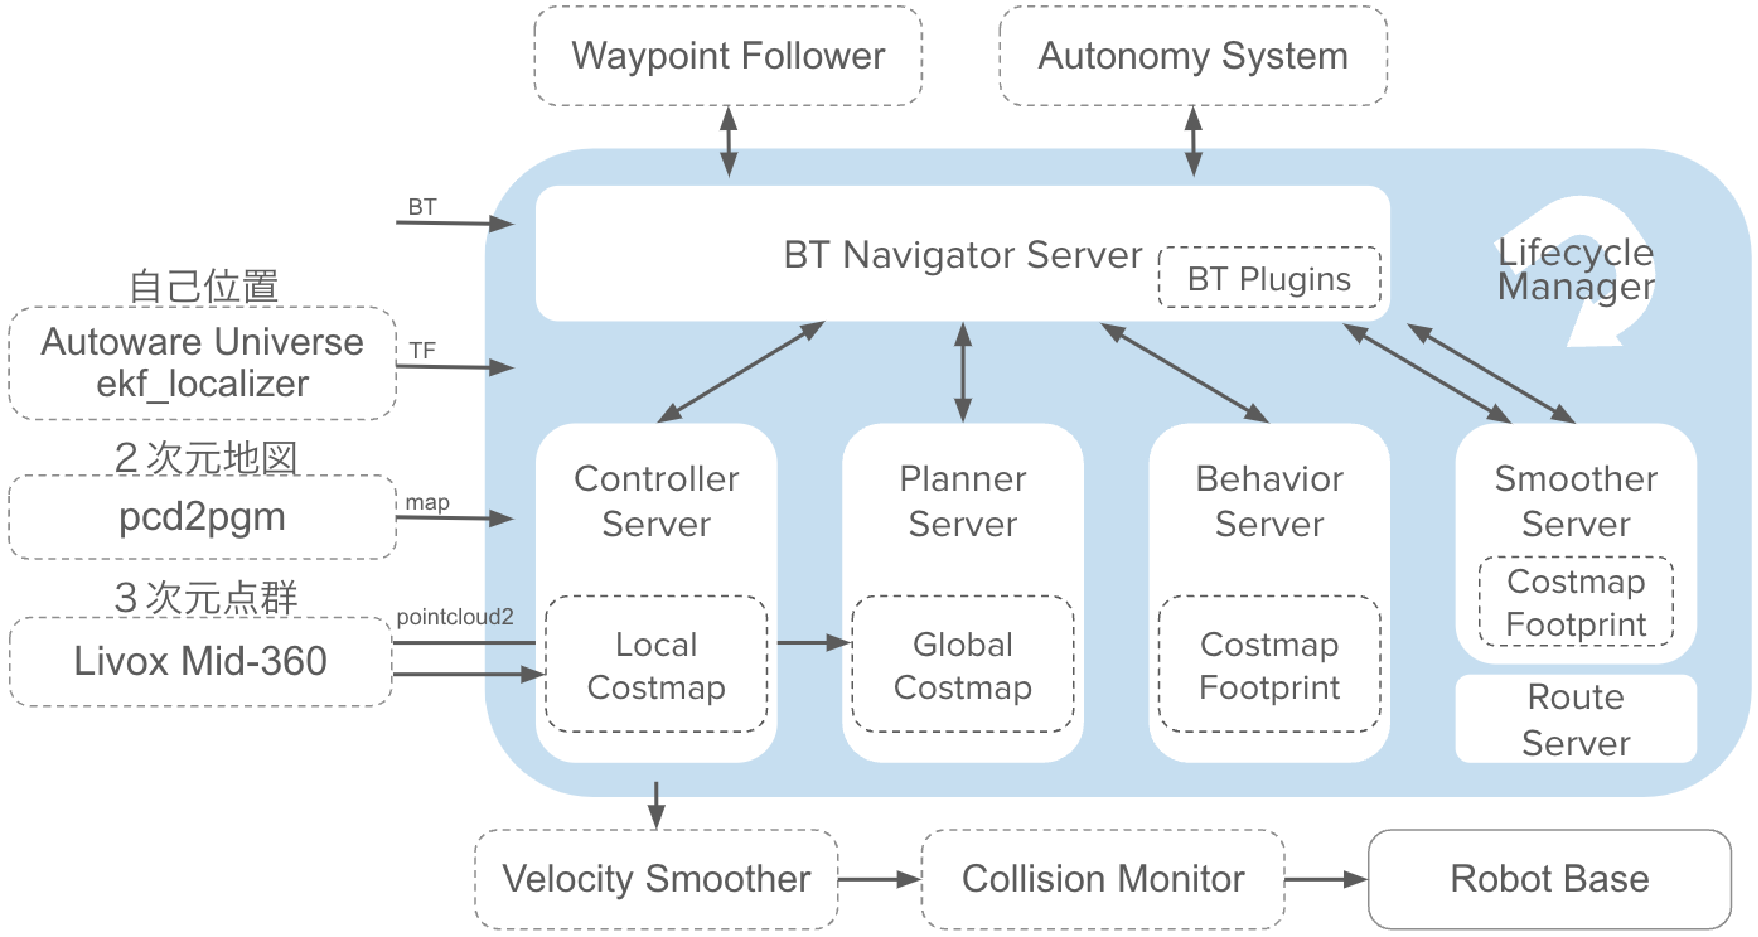
\includegraphics[width=1.0\linewidth]{figs/mugimaru_system.pdf}
    \caption{むぎまるチームのシステム構成}
    \label{fig:mugimaru_system}
  \end{center}
\end{figure}

%\begin{figure}[h]
%  \begin{center}
%      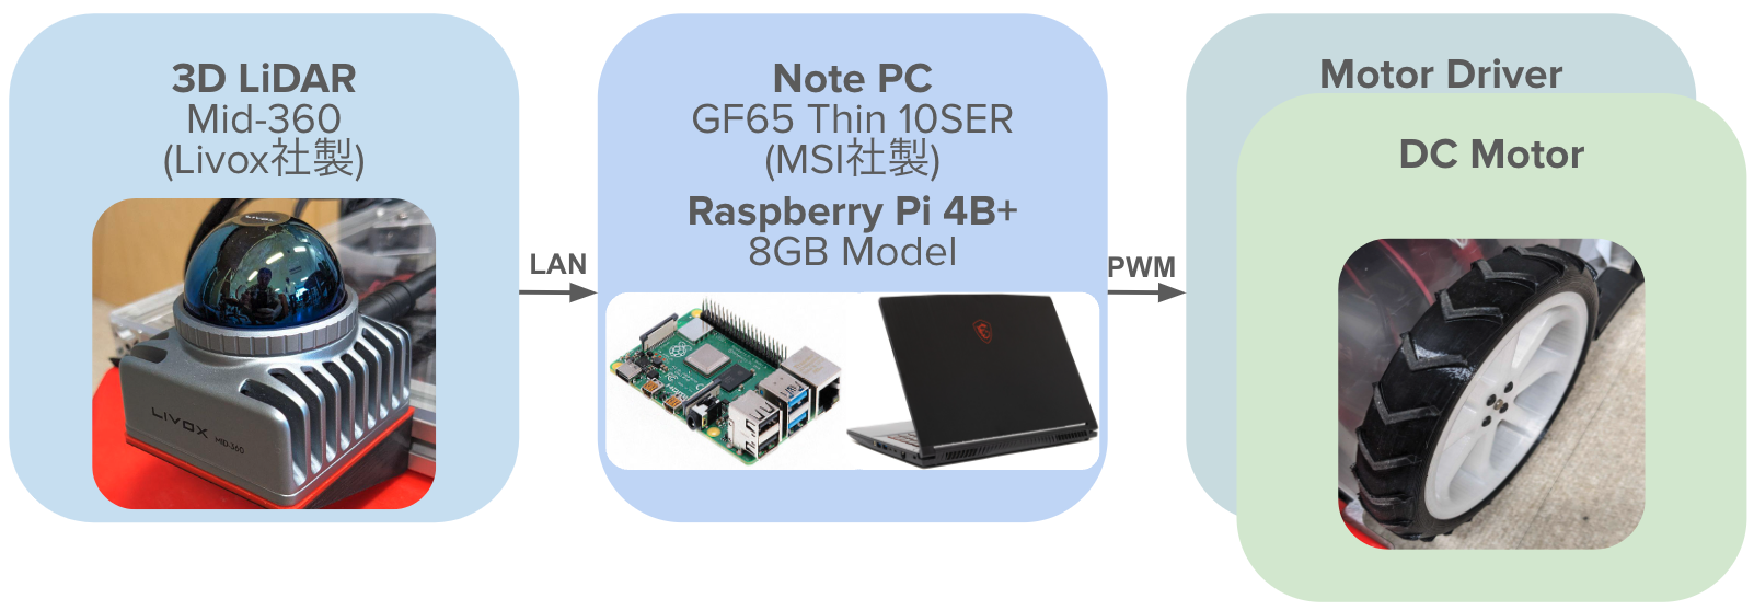
\includegraphics[width=1.0\linewidth]{figs/mugimaru_hard.pdf}
%      \caption{むぎまるチームのハードウェア構成}
%      \label{fig:mugimaru_hard}
%  \end{center}
%\end{figure}


%\section{本走行でのリタイアの原因}
\section{本走行の結果}

つくばチャレンジ2023での本走行の結果を表\ref{MainRun}に示す。

\begin{table}[H]
  \caption{各チームの本走行の結果}
  \label{MainRun}
  \begin{tabular}{|c|c|p{4.0cm}|}
    \hline
    チーム         & 走行距離 & リタイアの理由                                                                                             \\
    \hline
    ツナチーム     & 440[m]   & 市役所前の横断歩道の横断後の障害物回避課題に失敗                                                           \\
    \hline
    たまチーム     & 133[m]   & 市役所西側曲がり角で坂道に車輪を取られ自己位置推定が破綻                                                   \\
    \hline
    むぎまるチーム & 380[m]    & 市役所西曲がり角通過後,停止中の他チームのロボットの左側面に,本チームのロボットの右側面が接触する形で衝突 \\
    \hline
  \end{tabular}
\end{table}

%@@@ここの2段落、中途半端なので3.1以降に入れるか、しっかり概要を説明する@@@
%ツナチームは確認走行区間を走りきったが、最後の障害物回避の課題で、
%障害物を回避できず衝突し、失敗した。

%たまチームについては、表の通り、
%坂道において車輪を取られてしまい失敗した。
%坂道周辺では植え込みを用いて自己位置推定を試みたが失敗してしまった。

\subsection{ツナチーム}
\subsubsection{本走行の結果}
ツナチームの本走行の結果は、確認走行区間の最後の課題である障害物回避を失敗したため、
440[m]という結果になった。障害物回避の課題までは、ある一箇所を除いて、終始安定して走行できていた。
その一箇所は、市役所の入口付近であり、点字ブロックの上を走行していたため
オドメトリに誤差が多くのりロボットの位置と推定位置が縦方向にずれてしまった。
そのまま自己位置推定が破綻すると思われたが、
カーブ時に自己位置推定側(MCL)が上手いこと誤差を修正したため危機を脱した。
上記の状況は、動画\cite{ike_nav_loc_youtube}の(22:45〜24:45)に映されている。

ツナチームは、7/15、7/16、11/4、11/8、11/9の計5日間、実験走行および本走行に参加した。
この中でも、ike\_navの動作確認に費やしたのは、最後の11/8、11/9である。
夏休みから開発してきたike\_navを11/7にロボット上で使える状態にした。
そのため、直前ギリギリまで勧めていた作業としては、まずまずの結果といえる。

\subsubsection{本走行・実験走行で見つかった課題}
\paragraph{障害物回避の不安定さ}
本走行時、ike\_navの障害物回避の機能には、バグが含まれていた。
A*によって障害物回避をするようなパスを生成し、それを追従することで障害物回避としていた。
このA*では、推定位置からゴールまでの最短経路を導出しつつ、障害物回避を行うために、
独自のヒューリスティック関数を実装した。
これが、うまく実装できていれば良かったのだが、距離が遠いほど障害物回避を回避しようとしなくなるような
実装となっていた。そのため今後は、障害物回避の安定のために、この重みの計算を見直し、修正をする予定である。

% \paragraph{尤度場、コストマップの作成に時間がかかる}
% ike\_navでは、尤度場とコストマップを自律走行を開始させる前に作成する処理がある。
% 地図としては、確認走行区間のみの情報しかないが、
% この処理に、1分ほどかかってしまっていた。
% これは、尤度場、コストマップの作成の実装に問題があるため、
% 作成部分の実装を見直し、修正をする予定である。
% @@@1分くらいいいんじゃない?@@@

\subsection{たまチーム}
\subsubsection{本走行・実験走行で見つかった課題}
\paragraph{ロボットの旋回による自己位置の破綻}


たまチームはつくばチャレンジEXでの屋内での自律走行を実施した。
その際、IMUを搭載していなかったため、
ナビゲーション中にロボットが人混みを避けようとして頻繁に旋回し、
自己位置が破綻するという課題が生じた。
この課題への対策としてIMUを実装し、
速度指令値から求めた角速度を積分した値であるヨー軸の角度を、
IMUから得られるヨー方向の角速度の積分値に置き換えた。
その結果、
ナビゲーション中には何度も障害物を回避しようとして旋回することがあったが、
これらの旋回が自己位置推定の破綻には繋がらなかったという結果が得られた。


IMUの搭載による効果は、
マッピングの際にも確認できた。
マップの取得では、
人がコントローラを用いてロボットを操作した。
IMUを搭載していなかった際には、
操作ミスやタイヤのスリップによる不要な旋回が原因で、
歪んだマップが生成されることがあった。
しかし、IMUの搭載によりマップの歪みが減少した。
% マップの比較画像 %


\paragraph{マップの歪みが解消しきれていない課題}


IMUを搭載してマッピングを行ったが、
ループクローズが行われず、
結局歪んだマップしか取れなかった。
この問題に対処するため、
最終的にペイントツールを使用して人力で歪みを修正した。
しかし、これは根本的な解決ではなく、
問題の原因を究明し、
本質的な解決策を見つける必要がある。

\subsection{むぎまるチーム}
\subsubsection{本走行・実験走行で見つかった課題}

むぎまるチームの本走行・実験走行で見つかった課題は,障害物回避の失敗,3次元地図と2次元地図のズレ,消費電力の大きさである.
障害物回避の失敗についてはTable 1のとおりである.
本チームでは自己位置推定に使用する地図には,3次元点群地図を使用し,ナビゲーションには2次元の占有格子地図を使用している.
2次元の占有格子地図は3次元地図を元に生成しているのだが,3次元上の障害物を2次元上に投影する際に,坂のある地形ではズレが生じる.
3次元点群地図では,ロール方向のズレと,ピッチ方向のズレが存在するため,必然的に2次元上に投影すると,平面方向に誤差が生じる.
本チームではロボットの動作確認を,あまり坂道の存在しない環境で行っていたため,つくばチャレンジでの環境と想定以上の差が生じてしまった.

消費電力については,むぎまるチームでは
ノートPCの消費電力が当研究室の他チームに比べて大きくなった。
3次元点群ベースの自己位置推定を行う負荷が、
その原因となった。2次元より3次元のセンサ処理の
負荷が大きくなることは仕方ないかもしれないが、
処理の軽量化も課題としたい。

%@@@大会で使わなかったけど開発したソフトウェアとか、研究成果をしっかり説明すること。@@@

\section{結言}
センサとしてLiDAR,IMUのみを搭載した小型ロボットでつくばチャレンジに参加した.
今回はROSのサポート終了に伴い,以前のシステムをROS 2に移行したソフトウェア構成で参加したことに加え,
IMUや3次元LiDARの追加,自作のナビゲーションスタックの使用など,例年とは異なる開発内容となった.
来年度は今年度の開発内容をもとに,見つかった課題への対策や,今回開発が間に合わなかった機能の追加をし,
小型ロボットでのコースの完走を目指す.

計算量の少なさにこだわらない別の試みとして,パーティクルの分布から,不確かさを考慮して行動決定する手法を実装したROSパッケージを作成している\cite{pfc}.
この手法を実用できると,自己位置推定の結果が不確かであれば,センシングできない縁石などの障害物から遠ざかって移動するなど,
よりロボットに柔軟に行動決定させることができる\cite{tonouchi2023}\cite{ueda2023JRM}.
%ロボットがゴールに向かうための時間コストを更新し続け,ロボットの行動を生成する手法を実装したROSパッケージを作成している。
%また,価値反復を移動ロボットの行動計画に適用すると、ロボットがとりうるすべての状態に対して最適な行動を計算することができる。
%価値反復は、ベルマン最適方程式を用いて、有限マルコフ決定過程における最適方策を正確に求めることができる手法である。

他にも,人混みなどの複雑な環境での自己位置推定の破綻を防ぐための研究を行っている\cite{}.
%この手法を実用できると,
%観測する情報を間引き,MCLに未知障害物を取り込ませないことで,つくばチャレンジなど
この研究は,地図にないような人混みなどの障害物を未知障害物とし,観測情報を間引くことによって未知障害物を含まない観測情報を自己位置推定に使用する手法を提案した.
この研究の実験では、つくばチャレンジ本走行でのスタート地点における人混みを模したシミュレーション上で,提案手法を実装した場合と実装していない場合でロボットを自律走行させた完走率を比較し,
実装した場合の方が完走率が高いことを確認した.
この手法の性能調査は、シミュレータ上のみで完結しているため、つくばチャレンジ本走行で使用して効果について調査したいと考えている。

%つくばチャレンジ走行時など,未知障害物の多い環境でも
%観測範囲を絞り,未知障害物をMCLに取り込ませないことで位置推定の破綻を抑える研究を行った.
%この手法を実用できると,





\cite{ikebeMECH}


\section*{謝辞}
つくばチャレンジ実行委員会,つくば市の皆様に感謝申し上げます.
上田研究室の新井亮大氏、登内リオン氏,松井大和氏,山崎政光氏,林原研究室の皆様には,つくばチャレンジ 2022 の参加にあたりご意見,ご協力頂き感謝申し上げます.
%↑上田整理。あと、著者に名前を連ねない人がいたらここに書くと良いです。

% 参考文献
% \small
\footnotesize
\begin{thebibliography}{99}
  \bibitem{ROS}
  Morgan Quigley {\it et al.}: ``ROS: an open-source Robot Operating System,''
  Open-Source Software workshop of the International Conference on Robotics and Automation、2009.

  \bibitem{ROS 2}
  Macenski, Steven {\it et al.}: ``Robot Operating System 2: Design, architecture, and uses in the wild,''
  Science Robotics, Vol. 7、No. 66, 2022.

  %\bibitem{fox2003}
  %Dieter Fox:
  %``Adapting the Sample Size in Particle Filters Through KLD-Sampling,''
  %International Journal of Robotics Research、Vol. 22、No. 12、pp. 985-1003、2003.

  %\bibitem{gutmann2002}
  %Jens-Steffen Gutmann and Dieter Fox:
  %``An Experimental Comparison of Localization Methods Continued,''
  %Proc. of the IEEE/RSJ International Conference on Intelligent Robots and Systems (IROS),pp. 454-459、2002.

  % \bibitem{ueda2002tdp}
  % 	Ryuichi Ueda {\it et al.}: 
  % ``Team description of Team ARAIBO,'' 
  % Proc. of 2002 International RoboCup Symposium、2002. 

  % \bibitem{ueda2004iros}
  % Ryuichi Ueda {\it et al.}: 
  % ``Expansion Resetting for Recovery from Fatal Error in Monte Carlo Localization -- Comparison with Sensor Resetting Methods,'' Proc.of IROS,pp.2481--2486,2004.

  % \bibitem{map2gazebo}
  % Shiloh Curtis: ``shilohc/map2gazebo'',\url{https://github.com/shilohc/map2gazebo} (last visit: 2021-12-31).

  % \bibitem{move_base}
  % Eitan Marder-Eppstein: ``move\_base,'' \url{http://wiki.ros.org/move_base} (last visit: 2021-12-31).

  %\bibitem{amcl}
  %Brian Gerkey: ``amcl,'' \url{https://wiki.ros.org/amcl} (last visit: 2021-12-31).

  %\bibitem{gmapping}
  %Brian Gerkey: ``gmapping,'' \url{http://wiki.ros.org/gmapping} (last visit: 2021-12-31).

  % \bibitem{GIMP}
  % GIMP.org: ``GIMP,'' \url{https://www.gimp.org/} (last visit: 2021-12-31).

  \bibitem{emcl2}
  Ryuichi Ueda: ``ryuichiueda/emcl2,''\url{https://github.com/ryuichiueda/emcl2} (last visit: 2024-01-01).

  \bibitem{emcl2_ros2}
  Ryuichi Ueda: ``CIT-Autonomous-Robot-Lab/emcl2\_ros2,''\url{https://github.com/CIT-Autonomous-Robot-Lab/emcl2_ros2} (last visit: 2024-01-01).

  \bibitem{pfc}
  Ryuichi Ueda: ``ryuichiueda/value\_iteration (amdp branch),''\\\url{https://github.com/ryuichiueda/value_iteration/tree/amdp} (last visit: 2022-12-12).

  %\bibitem{raspicat}
  %Ryuichi Ueda and Daisuke Sato: ``ja/raspicat,'' \url{https://wiki.ros.org/ja/raspicat} (last visit: 2021-12-31).

  %\bibitem{youtube}
  %BEIKE: ``つくばチャレンジ2022 実験走行 11/19 スタートからゴールまで自律移動(神の手4回),'' \url{https://www.youtube.com/watch?v=3gpjVhRIJDY} (last visit: 2022-12-12).

  % \bibitem{raspicat_rosbag}
  % Tatsuhiro Ikebe: ``uhobeike/raspicat\_rosbag,'' \url{https://github.com/uhobeike/raspicat_rosbag} (last visit: 2021-12-31).

  %\bibitem{池邉2021}
  %池邉 龍宏,曹 越,高橋 秀太,クルス ペレス アントニオ,林原 靖男,上田 隆一: 小型移動ロボットによるつくばチャレンジへの挑戦,第22回計測自動制御学会システムインテグレーション部門講演会,pp.3390-3393,2021.

  \bibitem{池邉2022}
  池邉 龍宏,内田 璃空,畑中 優一郎,臼井 温希,庄司 史門,松井 大和,山崎 政光,登内 リオン,林原 靖男,上田 隆一: Raspberry Pi のみを計算に用いる小型移動ロボットでのつくばチャレンジ 2022 参加レポート,つくばチャレンジ2022シンポジウム予稿集,2022.

  % \bibitem{上田2019}
  % 上田 隆一: ``詳解確率ロボティクス''、講談社、2019.

  %   \bibitem{上田2020}
  %  上田隆一,鈴木勇矢: 自己位置が不確かな状況における移動ロボットの危険回避行動の生成,第38回日本ロボット学会学術講演会予稿集,pp.RSJ2020AC2C2-02,オンライン開催,2020.

  % \bibitem{地図合成}
  % 川合隆太他: ``産業技術大学院大学における自律移動ロボット「産技大2号」の開発'',2019年度つくばチャレンジシンポジウム、pp.4-7、2020.

  \bibitem{RTshop}
  株式会社アールティ:``Raspberry Pi Cat 屋外でも動かせる中型2輪ロボット'',
  RT Robot Shop Products,\url{https://rt-net.jp/products/raspberry-pi-cat/} (last visit 2024-01-05)

  % \bibitem{aws2020}
  %   CIT自律ロボット研究室: ``AWSロボットデリバリーチャレンジで本研究室メンバーが優勝,'' \url{https://lab.ueda.tech/?post=20200915_aws_challenge} (last visit 2022-01-04)

  % \bibitem{学科サイト}
  %   千葉工業大学先進工学部未来ロボティクス学科: ``AWS Robot Delivery Challenge 2021 準優勝''、\url{https://www.robotics.it-chiba.ac.jp/j/?p=838} (last visit 2022-01-04)

  % \bibitem{つくばチャレンジロボット仕様}
  % つくばチャレンジ実行委員会事務局:``つくばチャレンジ 2021 ロボット仕様条件'',
  % \url{https://tsukubachallenge.jp/2021/regulations/specs} (last visit 2021-12-31)

  \bibitem{UST-30LX}
  北陽電機株式会社:``UST-30LX'',\url{https://www.hokuyo-aut.co.jp/search/single.php?serial=195#spec} (last visit: 2021-12-31).

  % \bibitem{Turtlebot3 Burger}
  % 株式会社ロボティズ: ``Turtlebot3 Burgerの仕様'',\url{https://emanual.robotis.com/docs/en/platform/turtlebot3/features/} (last visit: 2022-1-3).

  % \bibitem{つくばチャレンジ公式記録}
  % つくばチャレンジ実行委員会事務局:``つくばチャレンジ2021の走行結果'',
  % \url{https://tsukubachallenge.jp/2021/records/final} (last visit 2021-12-31)

  % \bibitem{出野畑中}
  %   畑中 優一郎,出野 廣太郎,上田 隆一:``Raspberry Pi 3BのみでRaspberry Pi Catのナビゲーション(屋内環境編)'',CIT自律ロボット研究室,\url{https://lab.ueda.tech/?post=20211210} (last visit 2022-01-02)

  \bibitem{ike_nav}
  Tatsuhiro Ikebe: ``uhobeike/ike\_nav,''\url{https://github.com/uhobeike/ike_nav} (last visit: 2024-01-10).

  \bibitem{ike_nav_detail}
  Qiita : ``自作ナビゲーションスタックでつくばチャレンジ2023に挑戦してみた話'',
  \url{https://qiita.com/BEIKE/items/f3ff141cc25d49c01363} (last visit 2023-1-10).

  \bibitem{fastlio}
  Ericsii: ``Ericsii/FAST\_LIO (ros2 branch),''\url{https://github.com/Ericsii/FAST_LIO.git} (last visit: 2023-11-19).

  \bibitem{autoware}
  The Autoware Foundation: ``autowarefoundation/autoware.universe,''\url{https://github.com/autowarefoundation/autoware.universe.git} (last visit: 2023-11-19).

  \bibitem{nav2}
  ROS Planning: ``ros-planning/navigation2 (humble branch),''\url{https://github.com/https://github.com/ros-planning/navigation2.git.git} (last visit: 2023-11-19).

  \bibitem{fox1999etal}
  D. Fox and others : ``Monte Carlo Localization: Efficient Position Estimation for Mobile Robots,''
  Proc. of AAAI, pp. 343-349, 1999.

  \bibitem{hart1968}
  Peter E. Hart and Nils J. Nilsson and Bertram Raphael : ``A Formal Basis for the Heuristic Determination of Minimal Cost Paths,''
  IEEE Transactions on Systems Science and Cybernetics, Vol. 4, No.2, pp. 100-107, 1968.

  \bibitem{dijkstra1959}
  E. W. Dijkstra : ``A Note on Two Problems in Connexion with Graphs,''
  Numerische Mathematik, Vol. 1, pp. 269-271, 1959.

  \bibitem{alberto2006}
  Bemporad, Alberto : ``Model Predictive Control Design: New Trends and Tools,''
  Proceedings of the 45th IEEE Conference on Decision and Control, pp. 6678-6683, 2006.

  \bibitem{ike_nav_loc_youtube}
  D. Fox and others : ``自作パッケージで屋外自律移動してみた in つくばチャレンジ2023(本走行)'',
  \url{https://www.youtube.com/embed/k9yxRKOCa14?si=c7ISmE1wH5W4BhgU&amp;start=1365} (last visit 2024-01-05)

  \bibitem{tonouchi2023}
  登内リオン, 池邉龍宏, 林原靖男, 上田隆一, “価値反復を用いた移動ロボットによる屋外ナビゲーション,” 
  Proc. of JSME Conf. on Robotics and Mechatronics (ROBOMECH), Article No.2P1-G06, 2023 (in Japanese). 

  \bibitem{ueda2023JRM}
  R. Ueda, L. Tonouchi, T. Ikebe, and Y. Hayashibara, “Implementation of Brute-Force Value Iteration for Mobile Robot Path Planning and Obstacle Bypassing,” 
  J. Robot. Mechatron., Vol.35 No.6, pp. 1489-1502, 2023.

  \bibitem{ikebeMECH}
  池邉龍宏, 林原靖男, 上田隆一, “未知障害物によるモンテカルロ自己位置推定の破綻を防ぐための観測範囲の制限と選択,” 
  Proc. of JSME Conf. on Robotics and Mechatronics (ROBOMECH), Article No.2A2-G06, 2023 (in Japanese). 
\end{thebibliography}
\normalsize

\clearpage

%\section{付録として、各実験走行でどんなことをやっていたかを書く?}
% 当チームは、9日間分のすべての実験走行会に参加した。
% 7月2日、7月23日は確認走行区間から信号あり横断歩道手前までの自己位置推定のテストを行った。
% 地図は昨年作ったものを使い、自己位置推定のパッケージにemcl2を使った。
% また、駅・公園エリアの地図作成のためのrosbagを取った。
% 9月17日、10月1日は駅・公園エリアの走行実験を行った。
% 走行エリアが増えたことに伴い地図の容量が増大し、4GBメモリのRaspberry Piでは処理できなかった。
% メモリの容量を増やし、地図の余白部分を削ることで駅・公園エリアが走行できるようになった。
% 10月22日、10月23日は信号あり横断歩道の横断の走行テストを行った。
% 通常の走行速度では青信号中に横断しきれなかったため、
% 信号あり横断歩道の横断中のみ走行速度を変えることで、青信号中に横断しきることができた。

\end{document}
